
% ==============================================================
% Introduction
% ==============================================================

\section{Introduction}
\label{sec: Introduction}

In bidirectional traffic, right- and left-hand traffic requires 
vehicles keep either to the right or the left side of the road, 
respectively.\cite{Draper_Geoff_1993} The first right-hand 
traffic law in United State dates back to 1792, applied to the 
Philadelphia and Lancaster Turnpike.
\cite{Weingroff_Richard_2014}

The right-hand traffic rule derives regulations on multi-lane 
freeways, which often requires drivers to drive in the 
right-most lane unless they are passing another vehicle, in 
which case they move one lane to the left, pass, and return 
to their former travel lane. The overtaking lane provides 
redundant convenience and safety for vehicles to pass others, 
but lowers freeway's traffic flow capability.

Different models may exist that provide a better trade-off 
among traffic flow, safety and convenience. This paper 
considers these three criteria, introduces a different 
freeway traffic model and analyses performances of the two 
models.



% ==============================================================
% Modeling
% ==============================================================

\section{Performance Evaluation}
\label{sec: Performance Evaluation}

Performance of a traffic rule is determined by the three 
criteria below: 

\paragraph{Safety} Average flow density and braking capability 
of vehicles, and lane speed limits, together affect the safety 
state of the freeway. Overtaking action will change local flow 
density and thus disturb the safety state. \textbf{Safety 
factor $\alpha$} is a value that measures how safe a vehicle 
or a lane is, and its value can be calculated from evaluation 
functions discussed at section \ref{sec: Safety Factor}.

\paragraph{Traffic Flow} The usage efficiency of a road is 
called the traffic flow. Such efficiency can be measured 
by the \textbf{traffic flow factor $\beta$}, detailed 
definition of which is found at section \ref{sec: Traffic 
Flow Factor}.

\paragraph{Convenience} In right- or left-hand traffic, 
overtaking lane is designed redundantly, to provide 
convenience for vehicles in hurry to pass others, or handle 
emergency. Freeways without overtaking lane give extra flow, 
but decrease convenience feature, which is neither described 
in safety nor in traffic flow factors. Hence definition of 
\textbf{convenience factor $\gamma$} is necessary, found at  
section \ref{sec: Convenience Factor}.


\section{Safety Factor $ \aleph $}
\label{sec: Safety Factor}

\subsection{Safe Distance Evaluation}
\label{sec: Safe Distance Evaluation}

On the freeway, if a vehicle suddenly slows down, the one 
behind may crash into it. Consequently, a statutory 
distance between each two adjacent vehicles is needed to 
avoid danger. For instance in China, the minimum distance 
is 100 meters between two vehicles on freeway of vehicle 
speed over 100 km/s; and 50 meters on road below 100 km/s.
\cite{PRC_State_Council_Decree_405}

A more precise evaluation model is established to enable 
analysis in continuous mathematics. Parameters required 
in this model are as below, and consider the figure 
\ref{fig: Safe distance model sketch}.

\begin{table}
\centering
\begin{tabular}{ll}
\hline
Parameter & Description\\
\hline
$a_1$ & Deceleration of the following vehicle \\
$v_1$ & Velocity of the following vehicle \\
$a_2$ & Deceleration of the leading vehicle \\
$v_1$ & Velocity of the leading vehicle \\
$v_0$ & Identical crash speed \\
$t_r$ & Reaction time of the driver \\
$L$   & the safe distance \\
\hline
\end{tabular}
\caption{Parameters for safe distance evaluation model}
\end{table}

\begin{figure}[h]
\label{fig: Safe distance model sketch}
\small
\centering
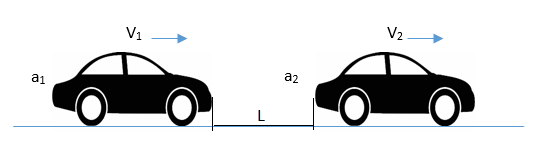
\includegraphics{situation.png}
\caption{Sketch diagram of safe distance evaluation model}
\end{figure}

Two possible cases of accident may happen:

\begin{itemize}

\item \textbf{The crash happens before when both vehicles 
are running.} To find the minimum safe distance between 
the two vehicles in this case, it is assumed that the 
distance between them is the minimum safe distance $ L $. 
The following vehicle's passing distance is the sum of 
decelerating and driver reaction distances. The sum is 
then the decelerating distance of the leading vehicle 
together with the minimum safe distance. This relation 
infers equation \ref{eq: Safe Distance 1 - 1}. The 
driver's reaction time is the gap between deceleration 
actions of the leading and following vehicles, which 
infers equation \ref{eq: Safe Distance 1 - 2}. One thing 
to notice, the crash speeds of both vehicles are identical. 
So the following vehicle's crash speed is large enough 
that crash can just happen, but small enough that the 
original distance is maximum to achieve safest minimum 
distance. To sum up in mathematical language, when
\begin{displaymath}
\frac{v_1}{a_1} + t_r < \frac{v_2}{a_2}
\end{displaymath}
two equations are inferred that 
\begin{eqnarray}
& \frac{v_1^2 - v_0 ^ 2}{2a_1} + v_1 t_r = L + \frac{
v_2 ^ 2 - v_0 ^ 2}{2a_2} &
\label{eq: Safe Distance 1 - 1}\\
& \frac{v_1 - v_0}{a_1} = \frac{v_2 - v_0}{a_2} - t_r &
\label{eq: Safe Distance 1 - 2}
\end{eqnarray}

\item \textbf{The following vehicle crashes into the 
leading vehicle after the leading one stops.} Similarly, 
the distance between two vehicles is assumed as the minimum 
safe distance $ L $. And the sum of decelerating and 
reaction distance is the safe distance adding the leading 
vehicle's deceleration distance, inferring equation 
\ref{eq: Safe Distance 2}. That is, when
\begin{displaymath}
\frac{v_1}{a_1} + t_r \geq \frac{v_2}{a_2}
\end{displaymath}
the distance relation is 
\begin{eqnarray}
& v_1 t_r + \frac{v_1 ^ 2}{2a_1} = L + \frac{v_2^2}{2a_2} &
\label{eq: Safe Distance 2}
\end{eqnarray}

\end{itemize}

By solving for the safe distance $ L $, the function of 
$ L $, the \textbf{safe distance evaluation function}, is 
obtained that 
\begin{equation}
L(a_1, a_2, v_1, v_2) = 
\left \{
\begin{array}{cl}
\dfrac{(a_1a_2t_r^2 + 2a_1t_rv_2 + v_1^2 - 2v_1v_2 + 
v_2^2)}{2(a_1-a_2)} & 
\dfrac{v_1}{a_1} + t_r < \dfrac{v_2}{a_2}\\
v_2 t_r + \dfrac{v_1 ^ 2}{2a_1} -\dfrac{v_2^2}{2a_2} & 
\dfrac{v_1}{a_1} + t_r \geq \dfrac{v_2}{a_2}
\end{array}
\right .
\end{equation}

This function describes the minimum safe distance that 
ensures two adjacent vehicles will just do or do not 
crash in given decelerations and velocities.


\subsection{Statutory Minimum Safe Distance}

To ensure absolute safety on freeway, statutory minimum 
safe distance is defined as the maximum value of safe 
distance $ L_{max} $ in all possible conditions. Denote 
the lower speed limit as $ v_{min} $, upper speed limit as 
$ v_{max} $, maximum deceleration of the vehicle with the 
worst braking system as $ a_{min} $, and that of the 
vehicle with the best braking system as $ a_{max} $. Then 
the statutory minimum safe distance
\begin{equation}
L_{max} = MAX(L(a_1,a_2,v_1,v_2))
\end{equation}
where $ a_{min} \le a_1,a_2 \le a_{max} $ and $ v_{min} 
\le v_1,v_2 \le v_{max} $.

To solve for the maximum value of $ L $, extrema are 
firstly inspected by finding the solution of the following 
partial differential equations simultaneously.
\begin{displaymath}
\left \{
\begin{array}{cl}
\dfrac{\partial L}{\partial{a_1}} = 0 \\
\dfrac{\partial L}{\partial{a_2}} = 0 \\
\dfrac{\partial L}{\partial{v_1}} = 0 \\
\dfrac{\partial L}{\partial{v_2}} = 0 \\
\end{array}
\right .
\end{displaymath}

This equation array has no solution, which indicates maximum 
at the domain boundary. If the leading vehicle runs at the 
lowest speed with the greatest deceleration, the following 
vehicle at the highest speed with the minimum deceleration, 
then the requested distance is the longest. In other words, 
$ L $ reaches the maximum when $ a_1 = a_{min} $, $ v_1 = 
v_{max} $, $ a_2 = a_{max} $ and $ v_2 = v_{min} $.

By substituting boundary values into the safe distance 
evaluation function, the condition below is satisfied that 
\begin{displaymath}
\dfrac{v_{min}}{a_{max}}  < \dfrac{v_{max}}{a_{min}} + t_r
\end{displaymath}

Hence the statutory minimum safety distance 
\begin{displaymath}
L_{max} = v_{min} t_r + \dfrac{v_{max} ^ 2}{2a_{min}} - 
\dfrac{v_{min}^2}{2a_{max}}
\end{displaymath}


\subsection{Safety Evaluation Function}

By substituting $ a_1 = a_{min} $, $ v_1 = v_{max} $ and 
$ v_2 = v_{min} $ to the safe distance evaluation function, 
the maximum-safe-distance function $ L_{max} $ with 
parameter $ a_2 $ is obtained that
\begin{displaymath}
L_{max}(a_2) = 
\left \{
\begin{array}{cl}
\dfrac{(a_{min}a_2t_r^2 + 2a_{min}t_rv_{min} + v_{max}^2 - 
2v_{max}v_{min} + v_{min}^2)}{2(a_{min}-a_2)} & 
\dfrac{v_{min}}{a_2}  \geq \dfrac{v_{max}}{a_{min}} + t_r \\
v_{min} t_r + \dfrac{v_{max} ^ 2}{2a_{min}} - \dfrac{
v_{min}^2}{2a_2} & \dfrac{v_{min}}{a_2}  < \dfrac{v_{max}}
{a_{min}} + t_r
\end{array}
\right .
\end{displaymath}

The function $ L_{max}(a_2) $ is a piecewise function, and 
its splitting point is 
\begin{displaymath}
K = \dfrac{v_{min}}{\dfrac{v_{max}}{a_{min}} + t_r}
\end{displaymath}

After substituting $ K $ to two function pieces, denoted by 
$ L_{max_1} $ and $ L_{max_2} $ respectively, it is found 
that 
\begin{equation}\label{eq: Function L - Continuity}
L_{max_1}(K) = L_{max_2}(K)
\end{equation}
which shows the \textbf{continuity} of the function 
$ L_{max} $.

And since 
\begin{equation}
\left \{
\begin{array}{cl}
L_{max_1}'(a_2) > 0 \\
L_{max_2}'(a_2) > 0
\end{array}
\right .
\end{equation}
The \textbf{monotonicity} of $ L_{max} $ is proved.

Thus the reversed function $ a2(L) $ exists, and it can 
be expressed as followed.
\[ a_2(l) = \begin{cases}
-\dfrac{v_{max}^2 - 2v_{max}v_{min} + 2a_{min}t_rv_{max} + v_{min}^2 - 2a_{min}t_rv_{min} - 2la_{min}}{a_{min}t_r^2 + 2l}, 
\\

\quad l \leq \dfrac{v_{max}^2 - v_{max}v_{min} + 2v_{max}a_{min}t_r - a_{min} v_{min}t_r}{2a_{min}}\\
\dfrac{a_{min}v_{min}^2}{v_{max}^2 + 2a_{min}t_rv_{max} - 2la_{min}}, \quad  l > \dfrac{v_{max}^2 - v_{max}v_{min} + 2v_{max}a_{min}t_r - a_{min} v_{min}t_r}{2a_{min}}
\end{cases}\]

\paragraph{\emph{Assumptions}} The driver press the brake 
always with strength that follows Gaussian distribution, 
where $\mu = \frac{a_{max}}{2}$, $\sigma = \frac{1}{4}\mu$, 
for $p(0 < a_2 < \frac{1}{4} \mu)$ and $p(\frac{7}{4} \mu 
< a_2 < 2\mu)$ is rare. And the brake strength directly 
determines a vehicle's deceleration, which means 
\begin{equation}
dp(a_2;\mu=\dfrac{a_{max}}{2},\sigma=\dfrac{a_{max}}{8})
 = \dfrac{1}{\sqrt{2\pi}\sigma}\exp^{-\dfrac{(a_2-\mu)^2}
{2\sigma^2}}
\end{equation}

Since the conversion functions between $ a2 $ and 
$ L_{max} $ exist, the probability distribution of 
deceleration is one-to-one projected to the safe distance 
distribution. The nearer two vehicles are, the more 
dangerous they are. So the integral of safe distance's 
probability distribution is exactly the evaluation of 
the safety, which is called the safety factor $ \aleph $. 
Mathematically, the safety factor 
\begin{equation}
\alpha(L) = \int_{0}^{L}dp(x;\mu=\dfrac{a_{max}}{2},\sigma=\dfrac
{a_{max}}{8})dx
\end{equation}

The greater the safety factor is, the safer a vehicle is. 
And if the distance reaches statutory minimal safe distance, 
\begin{equation}
\alpha(L_{max}) = \int_{0}^{L_{max}}dp(x) \approx 1
\end{equation}


\begin{figure}[h]
\small
\centering
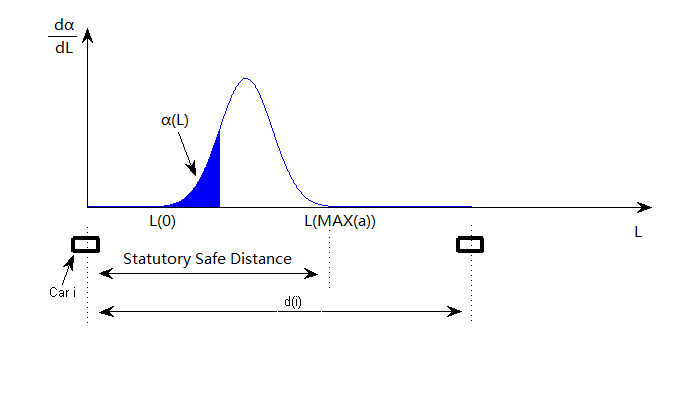
\includegraphics{draw_SafetyNormalDistribution_graph.png}
\caption{safety factor distribution} \label{fig: safety factor distribution}
\end{figure}




\section{Traffic Flow Factor $ \beta $}
\label{sec: Traffic Flow Factor}

Since the layout of the cars on the freeway is complicated, 
to simplify, we use a special model to discuss the 
relationship between the safety and traffic flow under the 
situation with and without the right-most rule.
\\
\emph{Assumption}
\begin{itemize}
\item $v$ and $\rho$ suits the Greenshield Model
%\item 车道上车的密度较小的时候,车的行驶
\end{itemize}

\begin{table}
\centering
\begin{tabular}{ll}
\hline
Parameter & Discription\\
\hline
$\rho $ & The traffic density\\
$\rho_j$ & The traffic density under the traffic jam condition. \\
&Under this condition, the distance between two adjant car is almost zero\\
$\rho_m$ & The traffic density when the the traffic flow is the highest.\\
$v_f$ & The velocity of the vehicle when the traffic density is small \\
$Q$ & Traffic flow \\
%$N$ & The total number of the car on the freeway
\hline
\end{tabular}
\caption{Model parameter}
\end{table}


\paragraph{The relationship between $v$ and $\rho$ }
According to the Greenshield Model, the $v $and $\rho$ has such a 
relationship:

\begin{equation}
v = a - b\rho
\end{equation}
$a$ and $b$ are coefficients

\begin{itemize}
\item let $\rho = 0$,$v = v_f$,
we have $a = v_f$
\\
\item when the traffic density is highest, that is,
$\rho = \rho j$, $v = 0$,
we have $b = \frac{v_f}{k_j}$
\end{itemize}

Therefore, we have 
\begin{equation}
v = v_f(1 - \frac{\rho}{\rho_j})
\end{equation}

\begin{equation}
\rho = \rho_j(1 - \frac{v}{v_f})
\end {equation}

\paragraph{The relationship between $Q$ and $\rho$ }
\begin{equation}
Q = \rho v = v_f(\rho - \frac{\rho^2}{\rho_j})
\end{equation}
This function has such properties:

\begin{itemize}
\item $Q$ is a quadratic function. 
\item when $\frac{dQ}{d \rho} = 0$, 
$\rho = \frac{1}{2}\rho_j = \rho_m $
What's more, it passes through the origin.
\end{itemize}


%\item Without the right-most rule, there is no overtaking lane, vehicle can stay on either lane at any time.
%\item On the freeway, except the overtaking car, others are subject to the uniform distribution.
%\end{itemize}


\section{Convenience Factor $ \gamma $}
\label{sec: Convenience Factor}

Without the right-most rule, a vehicle can drive on both lane for a long time. Under this condition, the events will be more common that one car blocks another car. This means that overtaking will be difficult,
in other word, be less convenient. Therefore, the block can evaluate the performance of the traffic flow.
%block: 两张车并行
We take one overtaking as a unit to
analyze. 
\emph{Assumptions}
\begin{itemize}
\item There are two lanes, one is normal lanes,
and the other is designed for overtaking
\item The two cars on the normal lane are driving
with a constant speed $\bar{v}$
\item The overtaking car is driving with speed
$v$, $v > \bar{v}$
\end{itemize}

During the overtaking
process, we find the condition which
is impossible to overtake, the situation
is discription in the figure as follow.

\begin{table}
\centering
\begin{tabular}{ll}
\hline
Parameter & Meaning\\
\hline
$s$ & the length of a car \\
$l$ & the safe distance \\
\hline
\end{tabular}
\caption{Model parameter}
\end{table}

\begin{equation}
w = - \frac{2s}{\bar{l} + s} 
\end{equation}
  
% ==============================================================
% Analysis
% ==============================================================

\section{Model Analysis}

\subsection{Traffic Flow}
\paragraph{Assumption}
\begin{itemize}
\item The distribution of the
vehicle velocity on the freeway
is normal distribution with mean
$\mu$ = 90 $km/h$. Since the speed 
limits are ususally 60 $km/h$ and 120 $km/h$
\item We take the interval 70$km/h$ - 90 $km/h$
to analysis.
\item As on the freeway, the velocity spread from
60$km/h$ to 90$km/h$, we take 70$km/h$ as the point where the traffic density is the highest.
Under this situation, we assume that the distance between two adjacent cars are the
safe distance. To simplify, the safe distance
equals to 140$m$(The $l_{max}$ when speed spreads from 0 - 120 $km/h$, acceleration spreads from 0 - 8 $m/s^2$)
\end{itemize}

We have 
\begin{equation}
v = v_f(1 - \frac{\rho}{\rho_j})
\end{equation}
When $v = 70km/h$, every two adjacent cars keep the distance 140$m$. Therefore,
the traffic density 
$\rho_j = \frac{1000}{140} = 7.14$.
Thus, $v = 90 - 2.8 \rho$,
let v = 0, we have
$\rho_j$ = 32.14,
$Q = 90((\rho - \dfrac{\rho ^2}{32.14})$

Without the right-most rule, the traffic density
is actually as twice as the density without this
rule.
That is , $\rho$ $\rightarrow$ $\dfrac{\rho}{2}$

\begin{displaymath}
Q = 2v_f(\dfrac{\rho}{2} -\dfrac{\frac{\rho}{2}}{\rho_j})
= v_f(\rho - \dfrac{\rho^2}{2\rho _j})
\end{displaymath}

\begin{figure}[htbp]
\centering
\begin{minipage}{60pt}
\centering
	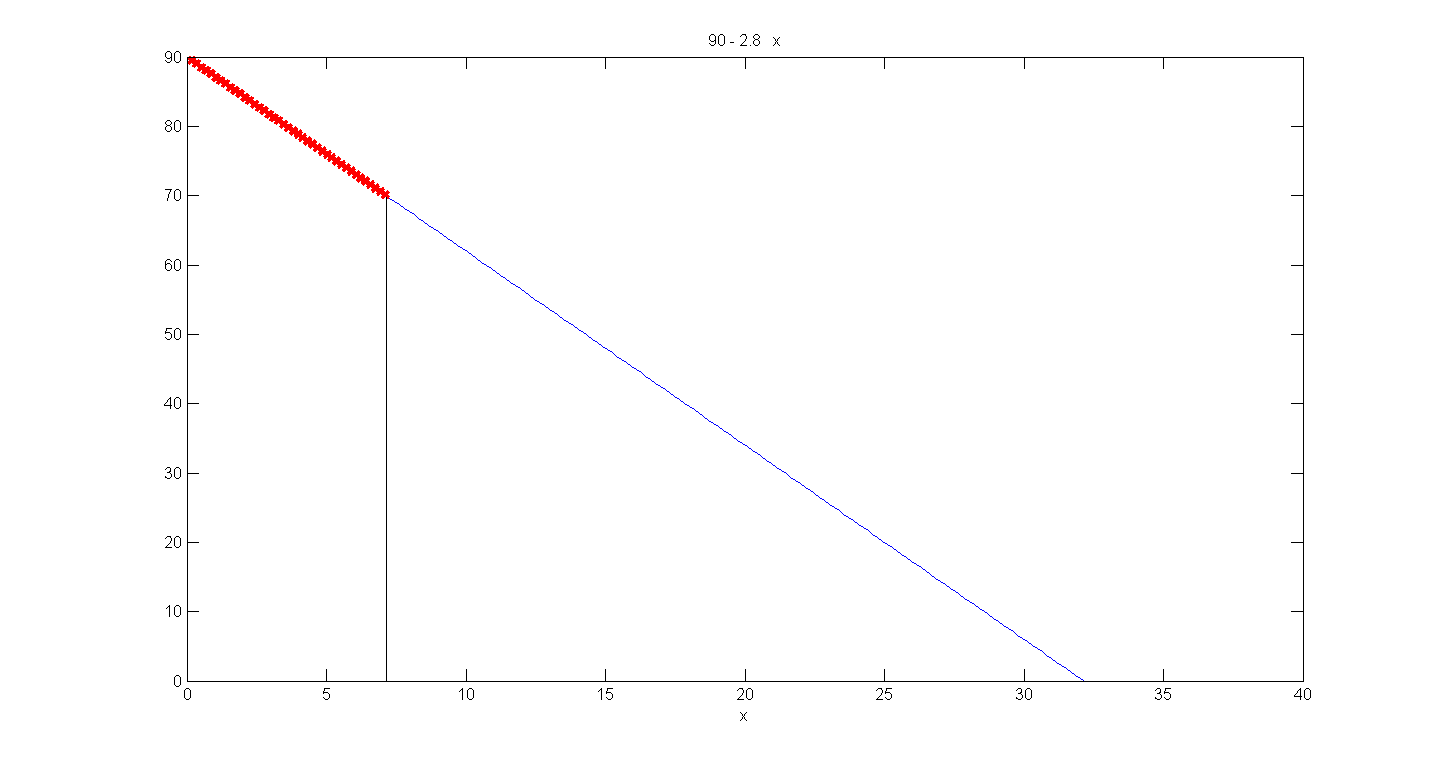
\includegraphics{v-p.png}
%\caption{$v = 90 - 2.8 \rho$}
\end{minipage}
\hspace{10pt}
\begin{minipage}{60pt}
\centering
 %label{fig: Safe distance model sketch}
%\small
	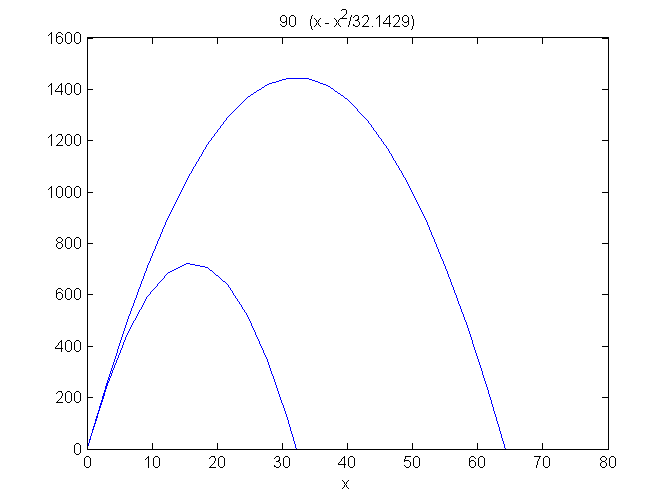
\includegraphics{Q-p.png}
	%\caption{Sketch diagram of safe distance evaluation model}
\end{minipage}
\end{figure}


% ==============================================================
% Conclusions
% ==============================================================

\section{Conclusions}



% ==============================================================
% Discussion
% ==============================================================

\section{Discussion}

\subsection{Strengths}

\paragraph{Safety Model}

\begin{itemize}
\item We consider the cars are the uniform distribution. However, it can hardly happen in the reality. Our model may have some error comparing with the actual situation.
\item We just consider a special situation where there is only one car overtaking. But in reality ,there may be a number of cars overtaking at the same time.
\end{itemize}

\paragraph{Traffic Flow Model}

\begin{itemize}
\item We assume the relationship between the velocity and traffic density suits the linear model. However, in reality, their relationship could just be negative correlation.
\item We assume when average distance is the statutory safe distance, the average  velocity is 70km/h. The reason why we assume the average velocity is 70km/h is that we believe when the average is the statutory safe distance, the average velocity should be low. And we just pick put a special velocity.
\end{itemize}

\paragraph{Convenience Model}
\begin{itemize}
\item We consider the cars are the uniform distribution.
\end{itemize}

\subsection{Weaknesses}
\paragraph{Safety Model}

\begin{itemize}
\item The safety model we get last get a certain function between the safety factor and traffic density. So it would be rather convenient to measure safety.
\item We considered the human judgment by probability we quantitatively calculated.
\end{itemize}

\paragraph{Traffic Flow Model}
\begin{itemize}
\item The traffic model we get last get a certain function between the traffic flow factor and traffic density. So it would be rather convenient to measure traffic flow.
\item We considered the relationship between the velocity and traffic density.
\end{itemize}

\paragraph{Convenience Model}
\begin{itemize}
\item The safety model we get last get a certain function between the convenience factor and traffic density. So it would be rather convenient to measure convenience.
\item We considered the advantage of the right-most rule. 
\end{itemize}
% ==============================================================
% References
% ==============================================================

\begin{thebibliography}{99}

\bibitem{Draper_Geoff_1993} Draper, Geoff (1993). "Harmonised 
Headlamp Design for Worldwide Application". Motor Vehicle 
Lighting. Society of Automotive Engineers. pp. 23-36.

\bibitem{Weingroff_Richard_2014} Weingroff, Richard. "On The 
Right Side of the Road". United States Department of 
Transportation. Retrieved 10 January 2014.

\bibitem{Mick_Hamer_1986} Hamer, Mick. "Left is right on the 
road", New Scientist, 25 December 1986 - 1 January 1987. No.
1540/1541, p.16.

\bibitem{PRC_State_Council_Decree_405} "Regulations for the Implementation of Law of the People's Republic of China on 
Road Traffic Safety". The State Council of the P.R.C., 30 
April 2004. Regulation No.80, Decree No.405.

\end{thebibliography}
